\documentclass[]{ltjtbook}

%%自作のB6tate.styを適用
\usepackage{B6tate} 

\title{吾輩は猫である} 
\author{夏目 漱石} 
\date{\today} 

\begin{document}
​ \maketitle %タイトルを挿入
​ \tableofcontents %目次を挿入

%以下に本文を書いていく。

\chapter*{はじめに\markboth{はじめに}{}}
\addcontentsline{toc}{chapter}{はじめに}

用紙B6サイズの縦書きの文章が書けます。

細かい調整をしたい場合は、B6tate.styをいじってください。

\oline{傍線}、そして、\kenten{傍点}……。

ダッシュ(―)を二つ。――。

〝ダブルミニュート(二重引用符)〟〝〟を「かっこ」と打てば出てくるように単語登録しておけばいいかも。

目次の挿入には「\$ lualatex 原稿」を2回実行する必要があります。

\begin{figure}
\begin{center}
\begin{minipage}<y>[htbp]{93mm} %
\centering
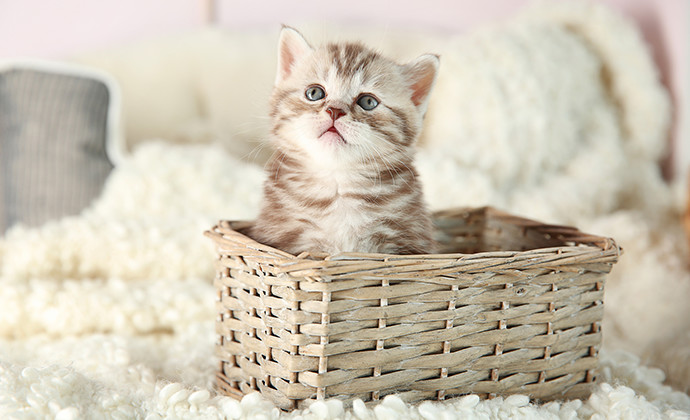
\includegraphics[width=93mm]{./pic/cat001.jpg} %
\caption{多賀山公園のネコ} %
\end{minipage}
\end{center}
\end{figure}



\chapter{見出し 吾輩は猫である。}

吾輩は猫である。名前はまだ無い。

どこで生れたかとんと見当がつかぬ。何でも薄暗いじめじめした所でニャーニャー泣いていた事だけは記憶している。吾輩はここで始めて人間というものを見た。しかもあとで聞くとそれは書生という人間中で一番\ruby{獰悪}{どう|あく}な種族であったそうだ。この書生というのは時々我々を捕えて煮て食うという話である。しかしその当時は何という考もなかったから別段恐しいとも思わなかった。ただ彼の掌に載せられてスーと持ち上げられた時何だかフワフワした感じがあったばかりである。掌の上で少し落ちついて書生の顔を見たのがいわゆる人間というものの見始であろう。この時妙なものだと思った感じが今でも残っている。第一毛をもって装飾されべきはずの顔がつるつるしてまるで\ruby{薬缶}{や|かん}だ。その後猫にもだいぶ逢ったがこんな片輪には一度も出会わした事がない。のみならず顔の真中があまりに突起している。そうしてその穴の中から時々ぷうぷうと煙を吹く。どうも咽せぽくて実に弱った。これが人間の飲む煙草というものである事はようやくこの頃知った。

この書生の掌の裏でしばらくはよい心持に坐っておったが、しばらくすると非常な速力で運転し始めた。書生が動くのか自分だけが動くのか分らないが無暗に眼が廻る。胸が悪くなる。到底助からないと思っていると、どさりと音がして眼から火が出た。それまでは記憶しているがあとは何の事やらいくら考え出そうとしても分らない。

ふと気が付いて見ると書生はいない。たくさんおった兄弟が一疋も見えぬ。肝心の母親さえ姿を隠してしまった。その上今までの所とは違って無暗に明るい。眼を明いていられぬくらいだ。はてな何でも容子がおかしいと、のそのそ這い出して見ると非常に痛い。吾輩は藁の上から急に笹原の中へ棄てられたのである。

ようやくの思いで笹原を這い出すと向うに大きな池がある。吾輩は池の前に坐ってどうしたらよかろうと考えて見た。別にこれという分別も出ない。しばらくして泣いたら書生がまた迎に来てくれるかと考え付いた。ニャー、ニャーと試みにやって見たが誰も来ない。そのうち池の上をさらさらと風が渡って日が暮れかかる。腹が非常に減って来た。泣きたくても声が出ない。仕方がない、何でもよいから食物のある所まであるこうと決心をしてそろりそろりと池を左りに廻り始めた。どうも非常に苦しい。そこを我慢して無理やりに這って行くとようやくの事で何となく人間臭い所へ出た。ここへ這入ったら、どうにかなると思って竹垣の崩れた穴から、とある邸内にもぐり込んだ。縁は不思議なもので、もしこの竹垣が破れていなかったなら、吾輩はついに路傍に餓死したかも知れんのである。一樹の蔭とはよく云ったものだ。この垣根の穴は今日に至るまで吾輩が隣家の三毛を訪問する時の通路になっている。さて邸へは忍び込んだもののこれから先どうして善いか分らない。そのうちに暗くなる、腹は減る、寒さは寒し、雨が降って来るという始末でもう一刻の猶予が出来なくなった。仕方がないからとにかく明るくて暖かそうな方へ方へとあるいて行く。今から考えるとその時はすでに家の内に這入っておったのだ。ここで吾輩は彼の書生以外の人間を再び見るべき機会に遭遇したのである。第一に逢ったのがおさんである。これは前の書生より一層乱暴な方で吾輩を見るや否やいきなり頸筋をつかんで表へ抛り出した。いやこれは駄目だと思ったから眼をねぶって運を天に任せていた。しかしひもじいのと寒いのにはどうしても我慢が出来ん。吾輩は再びおさんの隙を見て台所へ這い上った。すると間もなくまた投げ出された。吾輩は投げ出されては這い上り、這い上っては投げ出され、何でも同じ事を四五遍繰り返したのを記憶している。その時におさんと云う者はつくづくいやになった。この間おさんの三馬を偸んでこの返報をしてやってから、やっと胸の痞が下りた。吾輩が最後につまみ出されようとしたときに、この家の主人が騒々しい何だといいながら出て来た。下女は吾輩をぶら下げて主人の方へ向けてこの宿なしの小猫がいくら出しても出しても御台所へ上って来て困りますという。主人は鼻の下の黒い毛を撚りながら吾輩の顔をしばらく眺めておったが、やがてそんなら内へ置いてやれといったまま奥へ這入ってしまった。主人はあまり口を聞かぬ人と見えた。下女は口惜しそうに吾輩を台所へ抛り出した。かくして吾輩はついにこの家を自分の住家と極める事にしたのである。

\begin{figure}
\begin{center}
\begin{minipage}<y>[htbp]{93mm}
\centering
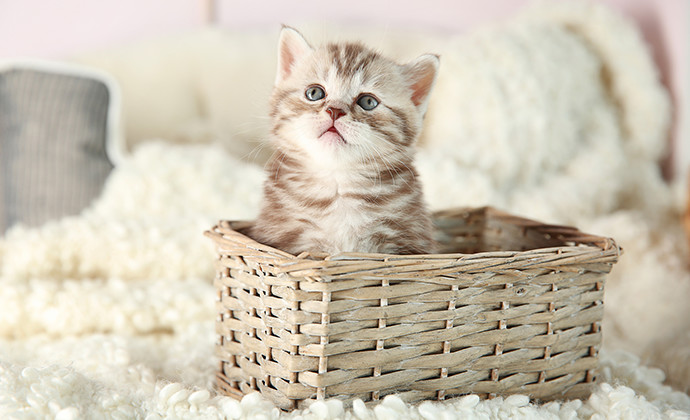
\includegraphics[width=93mm]{./pic/cat002.jpg}
\caption{吾輩は猫である。名前はまだ無い。}
\end{minipage}
\end{center}
\end{figure}

吾輩の主人は滅多に吾輩と顔を合せる事がない。職業は教師だそうだ。学校から帰ると終日書斎に這入ったぎりほとんど出て来る事がない。家のものは大変な勉強家だと思っている。当人も勉強家であるかのごとく見せている。しかし実際はうちのものがいうような勤勉家ではない。吾輩は時々忍び足に彼の書斎を覗いて見るが、彼はよく昼寝をしている事がある。時々読みかけてある本の上に涎をたらしている。彼は胃弱で皮膚の色が淡黄色を帯びて弾力のない不活溌な徴候をあらわしている。その癖に大飯を食う。大飯を食った後でタカジヤスターゼを飲む。飲んだ後で書物をひろげる。二三ページ読むと眠くなる。涎を本の上へ垂らす。これが彼の毎夜繰り返す日課である。吾輩は猫ながら時々考える事がある。教師というものは実に楽なものだ。人間と生れたら教師となるに限る。こんなに寝ていて勤まるものなら猫にでも出来ぬ事はないと。それでも主人に云わせると教師ほどつらいものはないそうで彼は友達が来る度に何とかかんとか不平を鳴らしている。

吾輩がこの家へ住み込んだ当時は、主人以外のものにははなはだ不人望であった。どこへ行っても跳ね付けられて相手にしてくれ手がなかった。いかに珍重されなかったかは、今日に至るまで名前さえつけてくれないのでも分る。吾輩は仕方がないから、出来得る限り吾輩を入れてくれた主人の傍にいる事をつとめた。朝主人が新聞を読むときは必ず彼の膝の上に乗る。彼が昼寝をするときは必ずその背中に乗る。これはあながち主人が好きという訳ではないが別に構い手がなかったからやむを得んのである。その後いろいろ経験の上、朝は飯櫃の上、夜は炬燵の上、天気のよい昼は椽側へ寝る事とした。しかし一番心持の好いのは夜に入ってここのうちの小供の寝床へもぐり込んでいっしょにねる事である。この小供というのは五つと三つで夜になると二人が一つ床へ入って一間へ寝る。吾輩はいつでも彼等の中間に己れを容るべき余地を見出してどうにか、こうにか割り込むのであるが、運悪く小供の一人が眼を醒ますが最後大変な事になる。小供は――ことに小さい方が質がわるい――猫が来た猫が来たといって夜中でも何でも大きな声で泣き出すのである。すると例の神経胃弱性の主人は必ず眼をさまして次の部屋から飛び出してくる。現にせんだってなどは物指で尻ぺたをひどく叩かれた。

\chapter{縦長の写真のテスト}

縦長の写真。

\begin{figure}
\begin{center}
\begin{minipage}<y>[htbp]{93mm}
\centering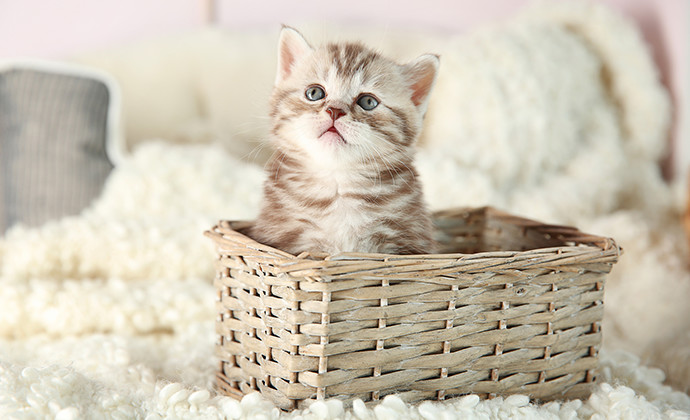
\includegraphics[width=93mm]{./pic/cat003.jpg}
\caption{黒猫}
\end{minipage}
\end{center}
\end{figure}

\chapter*{あとがき\markboth{あとがき}{}}
\addcontentsline{toc}{chapter}{あとがき}

あとがきとか、謝辞を書きましょう。

\rightline{広告鳥}

\begin{figure}
\begin{center}
\begin{minipage}<y>[htbp]{93mm}
\centering
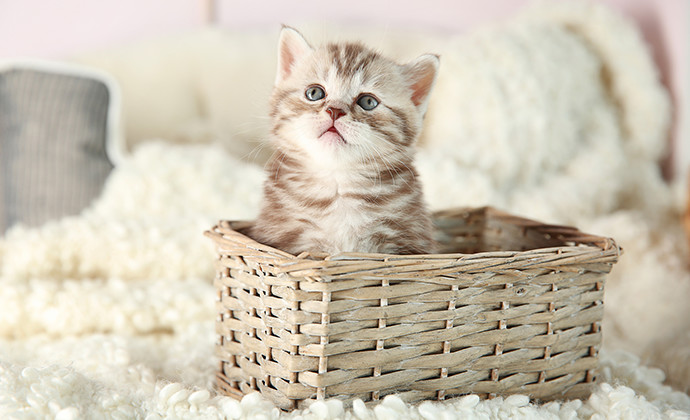
\includegraphics[width=93mm]{./pic/cat004.jpg}
\caption{}
\end{minipage}
\end{center}
\end{figure}

%奥付け
\clearpage
\thispagestyle{empty}
\begin{minipage}<y>[htpb]{93mm}
\begin{center}
​ \vspace{9cm} %奥付のページ上部からの位置

\begin{tabular}{l}
\multicolumn{1}{c}{\large{吾輩は猫である}}\\[3mm] %%タイトル
\hline
\\[-3mm]
\hspace{2mm}\normalsize{著\hspace{2mm}者}\hspace{5mm}夏目 漱石\\[0mm]  %%著者
\hspace{2mm}\small{発行日\hspace{5mm}\today}\\[0mm] %%発行日。「\today」のところに任意の日付を入れてもいい。
\hspace{2mm}\small{発行者}\hspace{5mm}{\small 広告鳥}\hspace{45mm}\scriptsize{※無断転載禁止}\\[-3mm]  %%発行者
\\\hline
\end{tabular}
\end{center}
\end{minipage}

\end{document}

%書き方メモ。コピペするときは頭のコメントアウト(%)を外して使う。
%
%「はじめに」とか「おわりに」など、章番号をつけたくないとき。
%\chapter*{はじめに\markboth{はじめに}{}}
%\addcontentsline{toc}{chapter}{はじめに}
%
%画像は以下をコピペ。
%\begin{figure}
%\begin{center}
%\begin{minipage}<y>[htbp]{93mm}
%\centering
%\includegraphics[width=93mm]{./pic/画像.jpg}%画像の幅と画像ファイルの指定
%\caption{キャプション}
%\end{minipage}
%\end{center}
%\end{figure}
%
